\section{Analysis of Fair-MAB in $K$-armed bandits}

For all of our results we assume that the means are upper bounded by a known constant $\mu^+$. If we don't do that we can use a forced exploration, but this would degrade some bounds in the scaling of $T$.
\begin{itemize}
	\item UCB allocation: works also for $\rho_\lambda=0$. Constant problem-dependent bandit regret, $\sqrt{T}$ fair regret.	
	\item LCB allocation: requires $\rho_\lambda>0$, constant problem-dependent fair regret, $\sqrt{T}$ bandit regret.
	\item Greedy allocation: $\rho_\lambda>0$, both regrets are in $\sqrt{T}$. 
\end{itemize}

TO-DO:
\begin{itemize}
	\item Check the ways to minimize $\sum \bP(\mu_k \notin [\LCB_{k,t}, \UCB_{k, t}])$ with a minimal confidence radius (should be fast, check e.g. the KL-UCB if I remember well) (minor).
	\item Check if there are some ways to avoid the dependency in $(\alpha_k)$ without degrading the performance (which is the case with forced exploration) (minor, I believe it's not possible).
	\item Check if we can avoid $\rho_\lambda>0$ and $\rho_\lambda^{-2}$ in the bounds for LCB and greedy. \textcolor{blue}{(Done and unified analysis)}
	\item Unfeasible case. (Done)
	\item Derive lower bounds. (in progress)
	\item See how these principles/proof techniques can be adapted for contextual case. (Most important point)
\end{itemize}


\subsection{Simulations}

% \subsubsection{Same algo for base bandit and fair allocation}
% \begin{figure}[H]
% 	\centering
% 	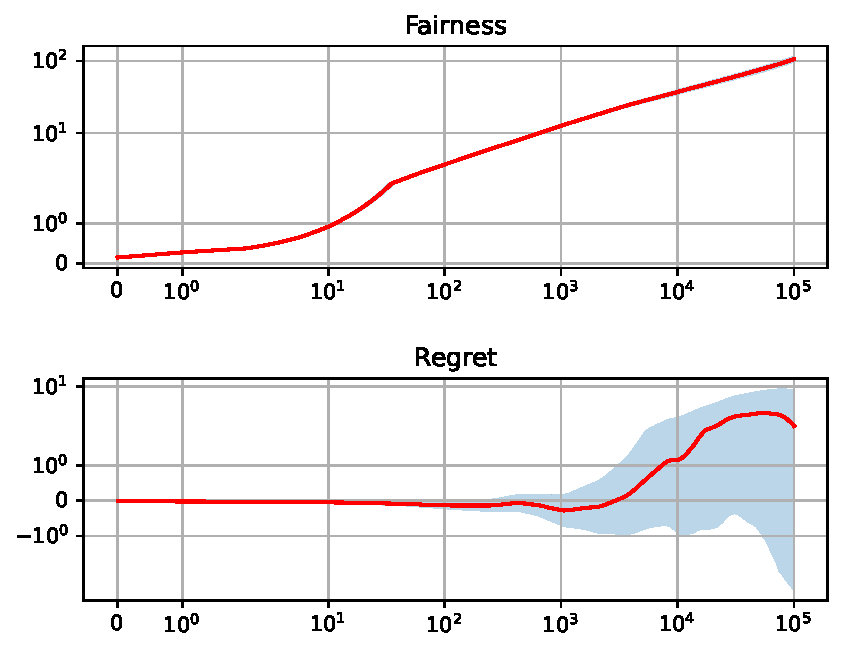
\includegraphics[width=0.8\textwidth]{../code/figures/mab_Greedy.pdf}
% 	\caption{Fair allocation and base bandit based on Greedy}
% 	\label{fig:}
% \end{figure}


% \begin{figure}[H]
% \centering
% 	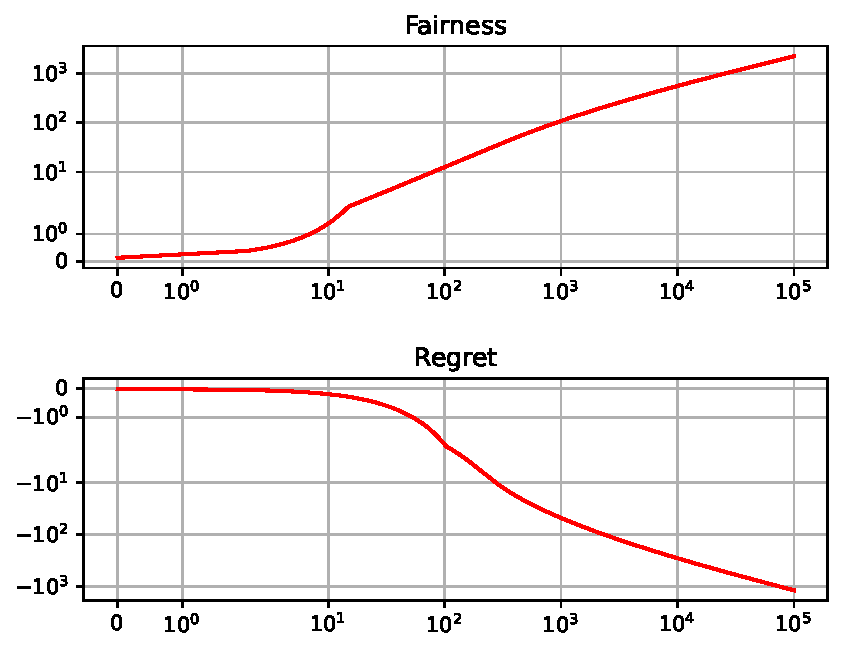
\includegraphics[width=0.8\textwidth]{../code/figures/mab_UCB.pdf}
% 	\caption{Fair allocation and base bandit based on UCB}
% 	\label{fig:}
% \end{figure}


% \begin{figure}[H]
% \centering
% 	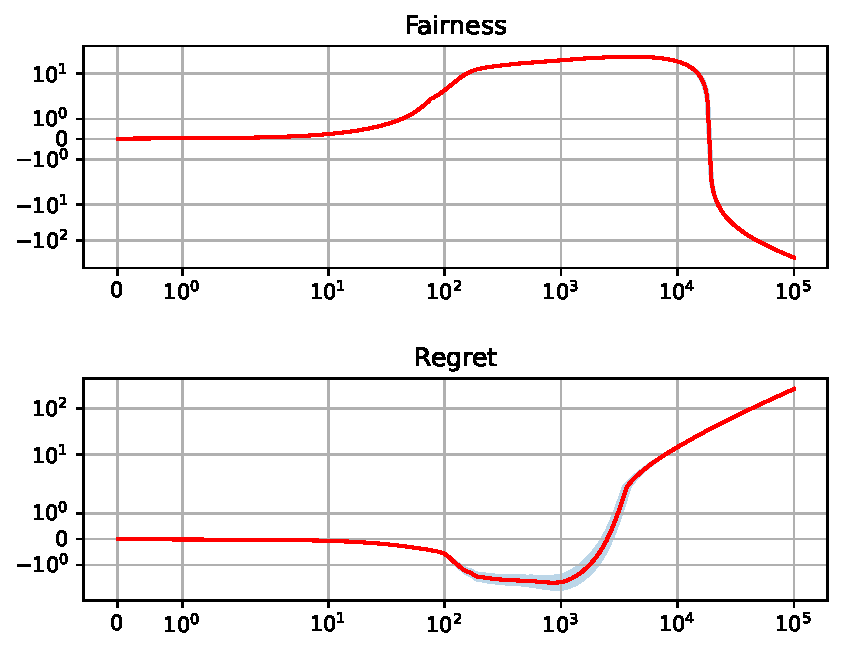
\includegraphics[width=0.8\textwidth]{../code/figures/mab_LCB.pdf}
% 	\caption{Fair allocation and base bandit based on LCB \hr{I believe this wierd behavior is because it takes long to find the correct arm, using Greedy or UCB for the base bandit should correct that}}
% 	\label{fig:}
% \end{figure}

\subsubsection{Greedy for base bandit, different fair allocations}

\subsubsection{UCB for base bandit, different fair allocations}

\subsection{Fair regret}

Consider Fair-MAB with any allocation. We first propose a generic upper bound that works under the three allocations that we proposed. We recall that we assume that $\max_j \mu_j \leq \mu^+$ for a known constant $\mu^+$, and that the problem is feasible so $\forall j \in [K], \wh q_{j,t}  \geq \alpha_j$ for some $\alpha_j>0$. For a time step $t$, consider the event \[\cG_t=\left\{ \forall k \in [K]\;:\; \mu_k \in [\LCB_{k, t}, \UCB_{k, t}], N_k(t)\geq \frac{\alpha_kt}{2}, \sum\frac{\lambda_j}{\wt \mu_{j,t}} \leq 1 \right\}\;,\]
 where we ommit the confidence levels in the notation for simplicity, but we will fix them later as a function of $t$. Consider an arm $k$, we want to upper bound $\cV_T^k \coloneqq \bE\left[\sum_{t=1}^T \left(\lambda_k-p_{k,t} \mu_k \right)\right]$.
 
We first write that 
\begin{align*}
\cV_T^k &\leq \bE\left[\sum_{t=1}^T \left(\lambda_k-p_{k, t} \mu_k \right)\right] \\
&
\leq  \underbrace{\bE\left[\sum_{t=1}^T \left(\lambda_k-\wh q_{k,t} \mu_k \right) \ind(\cG_t)\right]}_{V_1} + \underbrace{\bE\left[\sum_{t=1}^T \left(\lambda_k-p_{k, t} \mu_k \right) \ind(\bar \cG_t)\right]}_{V_2} \;. \\
\end{align*}


\paragraph{Upper bounding $V_1$} We first re-write $V_1$ as a function of $\wt \mu_{k, t}$ under $\cG_t$, 
\begin{align*}
V_1 & = \bE\left[\sum_{t=1}^T \left(\lambda_k- \frac{\lambda_k}{\wt \mu_{k, t}} \mu_k \right) \ind(\cG_t)\right] \\
& = \lambda_k \bE\left[\sum_{t=1}^T \left(\frac{\wt \mu_{k,t}-\mu_k}{\wt \mu_{k,t}}\right) \ind(\cG_t)\right]\;.
\end{align*}

Then, we remark that for the LCB allocation it simply holds that $V_1\leq 0$ since $\mu_k\geq \wt \mu_{k,t}$. Let us now consider the UCB allocation, under $\cG_t$ the term inside the expectation is non-negative and satisfies 
\[\frac{\wt \mu_{k,t}^{\UCB}-\mu_k}{\wt \mu_{k,t}^{\UCB}} \leq \frac{\UCB_{k,t}-\mu_k}{\mu_k} \leq \frac{\UCB_{k,t}-\LCB_{k, t}}{\mu_k} \;. \]
Furthermore, this bound also holds for the greedy allocation since the empirical mean also belong to the confidence interval. For these two allocations we thus obtain a bound that depend on the design of the confidence interval. 

We can give a more precise upper bound with the explicit form of the confidence interval. To provide a precise example, let us assume that the distributions are supported on $[0,1]$. For any $\delta>0$, Hoeffding's inequality states that 
\[\bP\left(|\wh \mu_{k, n}-\mu_k|\geq \delta \right)\leq 2e^{-2n\delta^2}\;, \]
so we can define for instance $\LCB_{k,t} = \wh \mu_k(t) - \sqrt{\frac{C\log(t)}{N_k(t)}} $ and $\UCB_{k,t} = \wh \mu_k(t) + \sqrt{\frac{C\log(t)}{N_k(t)}}$ for some $C>0$ to obtain a confidence level as a power of $t^{-1}$. Indeed, if holds that 
\begin{align*} \bP\left(|\wh \mu_k(t)- \mu_k|\geq \sqrt{\frac{C\log(t)}{N_k(t)}}, N_k(t)\geq \frac{\alpha_k t}{2} \right)&\leq \sum_{n=\frac{\alpha_k t}{2}}^t \bP\left(|\wh \mu_{k, n}- \mu_k|\geq \sqrt{\frac{C\log(t)}{n}}\right)  \\
&\leq 2 \sum_{n=\frac{\alpha_k t}{2}}^t t^{-2C}\leq \frac{2}{t^{2C-1}} \;,
\end{align*}

that we will use later in our analysis. For now, we simply use that this tuning ensures that \[\UCB_{k,t}-\LCB_{k, t} = 2\sqrt{\frac{C\log(t)}{N_k(t)}} \leq 2\sqrt{\frac{C\log(t)}{\alpha_k t}} \;, \]
again using that under $\cG_t$ it holds that $N_k(t)\geq \frac{\alpha_k}{2}t$. Plugging this into the upper bound on $V_1$, we obtain for the Greedy and UCB allocations that 

\[V_1 \leq \frac{\lambda_k}{\mu_k} \sum_{t=1}^T 2 \sqrt{\frac{C\log(t)}{\alpha_k t}} \leq 2\frac{\lambda_k}{\mu_k}\sqrt{\frac{CT\log(T)}{\alpha_k}}\;. \] 


\paragraph{Upper bounding $V_2$} A union bound provides that 
\begin{align*}
V_2 & \leq \lambda_k \sum_{j=1}^K \sum_{t=1}^T \bP(\mu_j \notin [\LCB_{j, t}, \UCB_{j, t}])  + \lambda_k \sum_{j=1}^K \sum_{t=1}^T\bP\left(N_j(t)\leq \frac{\alpha_j}{2}\right) \\
&+ \sum_{t=1}^T \bE\left[(\lambda_k - \wh q_{k,t}\mu_k)\ind\left(\forall j \in [K]; \mu_j \in [\LCB_{j, t}, \UCB_{j, t}], N_j(t)\geq \frac{\alpha_j}{2}t,  \sum_j \wh q_{j,t} \geq 1\right)\right] 
\end{align*}
 
First, we remark $\sum_{j=1}^K \sum_{t=1}^T \bP(\mu_j \notin [\LCB_{j, t}, \UCB_{j, t}])$ only depend on the confidence level of our LCB/UCBs. To make the sum converge we can for instance choose $\delta_t = 1/t^2$ and the first term of the upper bound of $V_2$ becomes $\cO(\lambda_k)$. With the Hoeffding's bound presented above, this condition is satisfied for $C=\frac{3}{2}$.

The second term can be upper bounded using that, at each time step $t$, the sampling probability of each arm $j$ is at least $\alpha_j$. Hence, $N_j(t)$ is stochastically dominated by a sum of i.i.d. Bernoulli random variables with probability $\alpha_j$, which leads to 
\begin{align*}
\sum_{j=1}^K \sum_{t=1}^T\bP\left(N_j(t)\leq \frac{\alpha_j}{2}\right) \leq \sum_{j=1}^K \sum_{t=1}^T e^{-t \kl\left(\frac{\alpha_j}{2}, \alpha_j\right)} \leq  \sum_{j=1}^K   \frac{1}{\kl\left(\frac{\alpha_j}{2}, \alpha_j\right)} \leq \sum_{j=1}^K\frac{2}{\alpha_j^2}\;,
\end{align*}
where $\kl$ denotes the Bernoulli KL-divergence. We get the intermediate result 

\[V_2 \leq \sum_{j=1}^K   \frac{1}{\kl\left(\frac{\alpha_j}{2}, \alpha_j\right)} + V_2'+ \cO(\lambda_k),  \]

with $V_2'=\sum_{t=1}^T \bE\left[(\lambda_k - \wh q_{k,t}\mu_k)\ind\left(\forall j \in [K]; \mu_j \in [\LCB_{j, t}, \UCB_{j, t}], N_j(t)\geq \frac{\alpha_j}{2}t, \sum_j \wh q_{j,t} \geq 1\right)\right]$.

We now upper bound the term $V_2'$, that depends on the choice of $\wt \mu_{k,t}$. Among our three allocations, the simplest case is UCB. Indeed, when all $(\mu_k)$ belong to their confidence bands it simply holds that  \[\sum_{j=1}^K \frac{\lambda_j}{\wt \mu_{j,t}^{\UCB}} \leq \sum_{j=1}^K \frac{\lambda_j}{ \UCB_{j,t}} \leq \sum_{j=1}^K \frac{\lambda_j}{ \mu_j}\;,\] so the UCB allocation is feasible and it directly holds that $V_2=\cO(\lambda_k)$ since the second term of its upper bound is in fact $0$.

If the allocation is LCB or greedy, the analysis is more involved, and we propose different paths depending  on the value of the feasibility gap $\rho_\lambda$: if $\rho_\lambda$ is positive, after some time normalization will not be needed with high probability, while if $\rho_\lambda=0$ (or is very small) it is likely to be needed for a long time.

By design the confidence bands also satisfy that $\wh \mu_j \in [\LCB_{j, t}, \UCB_{j, t}]$, it holds for all allocations that $\wt \mu_{j, t}\geq \mu_j- B_{j, t}$, with $B_{j,t} = \UCB_{j, t} - \LCB_{j, t}$. So, 

\begin{align*}
\sum_{j=1}^K \frac{\lambda_j}{\wt \mu_{j, t}} \leq \sum_{j=1}^K \frac{\lambda_j}{\mu_j - B_{j, t}} &= \sum_{j=1}^K \frac{\lambda_j}{\mu_j}\left(\frac{1}{1-\frac{B_{j, t}}{\mu_j}}\right) \\ &= \sum_{j=1}^K \frac{\lambda_j}{\mu_j} + \sum_{j=1}^K \frac{\lambda_j}{\mu_j}\times \frac{B_{j, t}}{1 - \frac{B_{j, t}}{\mu_j}} \\
& = 1-\rho_\lambda +\sum_{j=1}^K \frac{\lambda_j}{\mu_j}\times \frac{\frac{B_{j, t}}{\mu_j}}{1 - \frac{B_{j, t}}{\mu_j}}   \\
& \leq (1-\rho_\lambda)\left(1+ \max_{j\in[K]}\frac{\frac{B_{j, t}}{\mu_j}}{1 - \frac{B_{j, t}}{\mu_j}} \right) \;.  \\
\end{align*}

We now remember that we use this result under the event that each arm $j$ satisfies $N_j(t)\geq \alpha_j \frac{t}{2}$. The upper bound is increasing with $B_{j,t }$, which is itself upper bounded by its value for $N_j(t)= \alpha_j \frac{t}{2}$. With a Hoeffding's bound, the upper bound hence becomes 
\[\sum_{j=1}^K \frac{\lambda_j}{\wt \mu_{j, t}} \leq (1-\rho_\lambda)\left(1+ \max_{j\in[K]}\frac{\frac{2}{\mu_j}\sqrt{\frac{C\log(t)}{\alpha_j t}}}{1-\frac{2}{\mu_j}\sqrt{\frac{C\log(t)}{\alpha_j t}}} \right),\]
which is valid when $t$ is large enough so that the denominator is positive. We thus define the time \[t_\lambda(\CB)= \inf\left\{t \in \N: \; \max_j \frac{B_{j,t}}{\mu_j}\leq \frac{1}{2} | N_j(t)\geq \frac{\alpha_j}{2}t \right\}\;,\] so that for $t\geq t_\lambda$ we have that $B_{j,t}\leq \mu_j/2$. We can verify that $t_\lambda=\cO\left(\max_j\frac{1}{\alpha_j\mu_j^2}\log\left(\frac{1}{\alpha_j\mu_j^2}\right)\right)$.

Similarly, we can define the following deterministic time
\[t_\lambda'(\CB)= \inf\left\{t \in \N: \; \max_j \frac{B_{j,t}}{\mu_j}\leq \frac{\rho_\lambda}{2} | N_j(t)\geq \frac{\alpha_j}{2}t \right\}\;,\] so that for $t\geq \max\{t_\lambda(\CB), t_\lambda'(\CB)\}$ we have that $\sum_{j=1}^K \frac{\lambda_j}{\wt \mu_{j, t}} \leq 1$. We can also verify that $t_\lambda'(\CB)=\cO\left(\max_j\frac{1}{\alpha_j(\rho_\lambda \mu_j)^2}\log\left(\frac{1}{\alpha_j(\rho_\lambda \mu_j)^2}\right)\right)$, and is then scaling as $\rho_\lambda^{-2}$ if $\rho_\lambda>0$ and is infinite otherwise.

In the case where $\rho_\lambda>0$ we can simply write that \[V_2' \leq \max\{t_\lambda(\CB), t_\lambda'(\CB)\}= \cO\left(\max_j\frac{1}{\alpha_j(\rho_\lambda\mu_j)^2}\log\left(\frac{1}{\alpha_j(\rho_\lambda\mu_j)^2}\right)\right).\]

In the case where $\rho_\lambda=0$, we provide the following upper bound when $t \geq t_\lambda(\CB)$ and all the events considered in $V_2'$ hold, 
\begin{align*}
\lambda_k - \wh q_{k,t} \mu_k & = \lambda_k \left(1- \frac{\mu_k}{\wt \mu_{k, t}\left(1+2\max_j \frac{B_{j,t}}{\mu_j}\right)}\right) \\ 
& \leq \lambda_k \left(\frac{\wt \mu_{k,t}- \mu_k}{\wt \mu_{k, t}\left(1+2\max_j \frac{B_{j,t}}{\mu_j}\right)} +2\max_j \frac{B_{j,t}}{\mu_j} \right) \;.
\end{align*} 
For the LCB allocation the first term is negative under the events considered, while for the greedy allocation it can be upper bounded by $\frac{B_{k,t}}{\mu_k}$ just like $V_1$. The second term brings a $2\sum_{t=1}^T \max_j B_{j,t}/\mu_j$ to the regret, which gives $4\lambda_k\sqrt{\frac{C\log(T)T}{\min_{j \in [K]} (\alpha_j\mu_j^2)}}$ for the Hoeffding's bounds.

If we combine our two results, it holds for the greedy allocation that
\[ V_2' \leq \lambda_k\left(t_\lambda(\CB) + \left(t_\lambda'(\CB)-t_\lambda(\CB) \vee  \sum_{t=1}^T \left(\frac{B_{k,t}}{\mu_k}+2\max_{j\in[K]}B_{j,t}\right)\ind\left(N_k(t)\geq \alpha_k\frac{t}{2}\right) \right)\right) \;,   \]

which is asymptotically constant if $\rho_\lambda>0$ and scales in $\lambda_k \sqrt{\frac{T\log(T)}{\min (\alpha_j \mu_j^2 )}}$ if $\rho_\lambda=0$. Quite similarly, for the LCB allocation we obtain that
\[ V_2' \leq \lambda_k\left(t_\lambda(\CB) + \left(t_\lambda'(\CB)-t_\lambda(\CB) \vee 2\sum_{t=1}^T \max_{j\in[K]}B_{j,t}\ind\left(N_k(t)\geq \alpha_k\frac{t}{2}\right) \right)\right)  \;.   \]

\paragraph{Summary} We summarize our results, applying them for distributions with bounded supports and confidence intervals using Hoeffding's inequality. This way, we can exhibit a precise scaling in all the components of the problem. By upper bounding $V_1$ and $V_2$ we proved the following results when $\rho_\lambda>0$. 

For the LCB allocation,
\hr{$V_1$ decreases linearly while $V_2$ is constant, this means the fairness regret decreases linearly, we obtain negative fairness regret for LCB which is consistant with the simulations.
}

	\[\cV_T \leq \left(\max_{k \in K}\lambda_k\right) \left( K \sum_{t=1}^{+\infty} \frac{1}{t^2} + \sum_{j=2}^K\frac{1}{\kl\left(\frac{\alpha_j}{2}, \alpha_j\right)} + \cO\left(\max_j\frac{2}{\alpha_j(\rho_\lambda \mu_j)^2}\log\left(\frac{2}{\alpha_j(\rho_\lambda \mu_j)^2}\right)\right)\right) \;, \]
so the fair regret is upper bounded by a problem-dependent constant. 

For the greedy allocation, 
	\begin{align*} \cV_T \leq \max_{k\in K} &\left(\frac{2\lambda_k}{\mu_k}\sqrt{\frac{C T \log(T)}{\alpha_k}}+ \lambda_k\left(K \sum_{t=1}^{+\infty} \frac{1}{t^2} + \sum_{j=2}^K\frac{1}{\kl\left(\frac{\alpha_j}{2}, \alpha_j\right)} \right.\right. \\
	& \left.\left. + \cO\left(\max_j\frac{2}{\alpha_j(\rho_\lambda \mu_j)^2}\log\left(\frac{2}{\alpha_j(\rho_\lambda \mu_j)^2}\right)\right)\right)\right) \;. \end{align*}
\hr{I think this is shoting ourselves in the foot, if we cannot prove that Greedy has better fairness than UCB then let's remove Greedy.}

And for the UCB allocation, 
		\begin{align*} \cV_T \leq \max_{k\in K} &\left(\frac{2\lambda_k}{\mu_k}\sqrt{\frac{C T \log(T)}{\alpha_k}}+ \lambda_k\left(K \sum_{t=1}^{+\infty} \frac{1}{t^2} + \sum_{j=2}^K\frac{1}{\kl\left(\frac{\alpha_j}{2}, \alpha_j\right)}\right)\right) \;. \end{align*}
Furthermore, when $\rho_\lambda$ is small or $0$ the term in $\rho_\lambda^{-2}$ can be replaced by the upper bounds on $V_2'$ presented above, scaling (if we consider $T$ only) in $\sqrt{T\log(T)}$. The fact that it is possible in some cases to get a problem-dependent constant upper bound for the LCB allocation proves that the Fair Bandit equipped with this allocation will satisfy the fairness constraint faster than with the other approaches on average. On the other hand, UCB and Greedy both provide a bound of order $\cO(\sqrt{T\log(T)})$ in all cases. However, the second-order term of UCB is better since it does not depend on the feasibility gap. This has another advantage, which is that the upper bound for UCB do not depend on $\mu_k$ (since $\lambda_k/\mu_k \leq 1$) but only on $(\alpha_j)_{j \in [K]}$ (more precisely in $\max_j \alpha_j^{-2}$).

\hr{Currently, the bound does not behave well when $\lambda_{k} \to 0$, since this implies $\alpha_{k} \to 0$. This should not happen since all allocations should be fair when $\lambda_k \to 0$.}

\subsection{Bandit regret}

We know upper bound the bandit regret for the three instances of Fair MAB that we considered. Similarly to what we did in previous section, we consider the following good event
 \[\cG_t=\left\{ \forall k \in [K]\;:\; \mu_k \in [\LCB_{k, t}, \UCB_{k, t}], N_k(t)\geq \frac{\alpha_k t}{2} \right\}\;.\]
 The main difference is that here it is not necessary to check the value of $\sum_j \frac{\lambda_j}{\wt \mu_{j,t}}$, since in any case it holds that $p_{k,t}\leq \frac{\lambda_k}{\wt \mu_{k,t}}$. This will simplify the analysis of $\bP(\bar \cG_t)$ compared to previous section.


We denote by $\cR_{T,k}$ the contribution of a sub-optimal arm $k$ to the bandit regret, and first write that 
\begin{align*}
\cR_{T,k} &= \bE\left[\sum_{t=1}^T (p_{k,t} - p^\star_k)(\ind(\cG_t)+\ind(\bar \cG_t))\right]\Delta_k \\
& \leq \sum_{t=1}^T (1-p_k^\star) \bP(\bar \cG_t) + \bE\left[\sum_{t=1}^T (p_{k,t} - p_k^\star)\ind(\cG_t)\right] \Delta_k \;.
\end{align*}

We can use our results from previous section, obtaining that for all allocations 
\[\sum_{t=1}^T \bP(\bar \cG_t) \leq K \sum_{t=1}^{+\infty} t\delta_t + \sum_{j=2}^K\frac{1}{\kl\left(\frac{\alpha_j}{2}, \alpha_j\right)}\;, \]
where $\delta_t$ is the confidence level chosen for each interval $[\LCB_{k,t}, \UCB_{k,t}]$. We can hence focus on upper bounding $\cS_{T, k} \coloneqq \bE\left[\sum_{t=1}^T (p_{k,t} - p_k^\star)\ind(\cG_t)\right]$. 

Using Equation~\eqref{eq::sampling_prob}, we obtain that 
\begin{align*}\cS_{T,k} &= \bE\left[\sum_{t=1}^T (\wh q_{k, t} + (1-\sum_j \wh q_{j, t}) \ind(k_t=k) - p_k^\star)\ind(\cG_t)\right] \\
& \leq   \underbrace{\bE\left[\sum_{t=1}^T (\wh q_{k, t}-p_k^\star) \ind(\cG_t)\right]}_{\cO_{ T,k}} + \underbrace{\bE\left[\sum_{t=1}^T (1-\sum_j \wh q_{j, t}) \ind(k_t=k)\ind(\cG_t)\right]}_{\cB_{T,k}} \;.
\end{align*}

This upper bound separates the regret due to the allocation ($\cO_{T,k}$) and the regret due to the base bandit ($\cB_{T,k}$). We now further upper bound these two terms separately.

\paragraph{Upper bounding $\cO_{T, k}$} The regret due to the allocation can be upper bounded very similarly as the term $V_1$ of the fair regret (see previous section). Indeed, we can re-write $\cO_{T,k}$ as 
\[\cO_{T,k} =\bE\left[\sum_{t=1}^T \frac{\lambda_k}{\mu_k}\left(\frac{\mu_k-\wt \mu_{k, t}}{\wt \mu_{k, t}} \wedge 1 \right) \ind(\cG_t)\right] \;.  \]

Under $\cG_T$, the UCB allocation ensures that $\wt \mu_{k, t}\geq \mu_k$, so $\cO_{T,k}=0$. 
\hr{Actually, this is where we see negative regret appear for UCB since it will be negative linear regret against positive square root}

For the two other policies it is easy to verify that 
\[ \cO_{T,k} \leq \bE\left[\sum_{t=1}^T \frac{\lambda_k}{\mu_k}\left(\frac{\UCB_{k, t}- \LCB_{k, t}}{\LCB_{k, t}}\wedge 1\right) \ind(\cG_t)\right].\]
We reuse $t_\lambda(\CB)$ from the previous section (for $t\geq t_\lambda(\CB)$, we have $\LCB_{k,t}\geq \frac{\mu_k}{2}$ if $N_k(t)\geq \frac{\alpha_k t}{2}$). It holds directly that 
\[\cO_{T,k} \leq \frac{\lambda_k}{\mu_k} \left(t_\lambda(\CB) + \frac{2}{\mu_k}\bE\left[\sum_{t=t_k}^T (\UCB_{k, t}- \LCB_{k, t}) \ind(\cG_T)\right] \right) \;. \]

As before, we can be more specific for Hoeffding's bounds, and obtain (see previous section for details) that
\[ \cO_{T,k} \leq 2\frac{p_k^\star}{\mu_k}\sqrt{\frac{T\log(T)}{\alpha_k}} + \cO\left(\frac{\lambda_k}{\alpha_k \mu_k^3}\log\left(\frac{4}{\alpha_k \mu_k^2}\right)\right)  \;. \]


\paragraph{Upper bounding $\cB_{T, k}$} \textcolor{blue}{I continue the proof for a UCB algorithm, the proof is actually straightforward for optimistic algorithms since the best arm is represented by its UCB. For other policies the analysis would be more involved: we would need to make sure that the best arm is sampled enough to have a good mean, so that the algorithm is well-performing. We would surely need for instance that the probability of playing the bandit is large enough (e.g larger than $\rho_\lambda/2$), and we would get in that case a factor $2/\rho_\lambda$ in front of the upper bound of the second-order term of the standard bandit regret.\\
Adapt the message in the main text depending on what we find.}

\hr{Ok here, I believe we should actually use UCB to choose the arm (depending on the values of $\lambda$) so that we always have a good behavior for the allocation of the arm.
Then, we can either choose UCB or LCB to focus on fairness or regret}

First, under $\cG_t$ we can provide a deterministic upper bound of $1-\sum_j \wh q_{j,t} $. Indeed,
\begin{align*}
1-\sum_j \wh q_{j,t} & \leq 1 - \sum_j \frac{\lambda_j}{\UCB_{j,t}} \\
& \leq 1- \sum_j \frac{\lambda_j}{\mu_j + B_{j,t}} \\
& \leq 1- \left(\sum_j \frac{\lambda_j}{\mu_j}\left(1- \frac{B_{j, t}/\mu_j}{1+B_{j,t}/\mu_j}\right) \right) \\
& \leq \rho_\lambda + \sum_j \frac{\lambda_j}{\mu_j^2} B_{j,t}\\
&\leq \rho_\lambda + (1-\rho_\lambda)\max_{j \in[K]} \frac{B_{j,t}}{\mu_j} \to \rho_\lambda \;.
\end{align*}

Hence, (to avoid painful term-by-term upper bounds involving $\max_{j \in[K]} \frac{B_{j,t}}{\mu_j}$) we state that \[\bE\left[\sum_{t=1}^T (1-\sum_j \wh q_{j, t}) \ind(k_t=k)\ind(\cG_t)\right] = \rho_\lambda \bE\left[\sum_{t=1}^T \ind(k_t=k)\ind(\cG_t)\right] + o\left(\bE\left[\sum_{t=1}^T \ind(k_t=k)\ind(\cG_t)\right]\right)\;, \]
so we now focus on upper bounding the term $\bE\left[\sum_{t=1}^T \ind(k_t=k)\ind(\cG_t)\right]$. We consider a UCB base bandit, that chooses $k_t = \argmax{} \UCB_{k, t}$. Even if the algorithm uses observations that were not necessarily collecting because of its policy, the analysis can be fully conducted following the proof steps of any standard analysis of a UCB policy.  We first write that

\begin{align*}
\bE\left[\sum_{t=1}^T \ind(A_{t+1}=k, \UCB_{k, t}\geq \max_j \UCB_{j, t}, \cG_t)\right] & \leq \bE\left[\sum_{t=1}^T \ind(A_{t+1}=k, \UCB_{k, t}\geq \UCB_{1, t}, \cG_t)\right] \\
& \leq \bE\left[\sum_{t=1}^T \ind(A_{t+1}=k, \UCB_{k, t}\geq \mu_1)\right] \;. \end{align*}

Classically, we then use that for $N_k(t)\geq \frac{2C}{\Delta_k^2} \log(t)$ we have that $\UCB_{k, t}\geq \mu_1 \Rightarrow \wh \mu_{k, t} \geq \mu_k + \frac{\Delta_k}{2}$, so we can obtain that 

\begin{align*}
\bE\left[\sum_{t=1}^T \ind(A_{t+1}=k, \UCB_{k, t}\geq \mu_1)\right] &\leq \frac{2C}{\Delta_k^2} \log(T) + \sum_{n=\frac{2C}{\Delta_k^2} \log(T)}^T \bP\left(\wh \mu_{k, n}\geq \mu_k + \frac{\Delta_k}{2}\right) \\
& \leq \frac{2C}{\Delta_k^2} \log(T) + \frac{2}{\Delta_k^2} \;.
\end{align*}

Note that this bound holds even if $\lambda_k=0$, which is expected since it is the standard upper bound of the regret of \texttt{UCB1}. We thus obtain the folklore results of $\cO(\log(T))$ problem-dependent bound and $\cO(\sqrt{T\log(T)})$ worst-case bound.

Interestingly, if $\lambda_k>0$ we can provide an alternative upper bound, that provides a constant problem-dependent upper bound. Indeed, we recall that under $\cG_t$ it holds that $N_k(t)\geq \alpha_k \frac{t}{2}$, and so the first term can in fact be replaced by $\frac{2C}{\Delta_k^2}\log(T)\wedge t_k$, where $t_k$ is defined as follows,
\[t_k = \inf\{t\in \N: \; \frac{\alpha_k}{2}t\leq \frac{2C}{\Delta_k^2} \log(t) \}= \cO\left(\frac{4C}{\alpha_k \Delta_k^2}\log\left(\frac{4C}{\alpha_k\Delta_k^2}\right)\right)\;.\]

Hence, in all generality we finally obtain that 
\begin{align*}
\bE\left[\sum_{t=1}^T \ind(A_{t+1}=k, \UCB_{k, t}\geq \mu_1, \cG_t)\right] &\leq t_k \wedge  \frac{2C}{\Delta_k^2}\log(T) + \frac{2}{\Delta_k^2} \;.
\end{align*}

Hence, if $\lambda_k>0$, the base bandit only adds a problem-dependent constant to $\cS_{T,k}$, however the worst-case bound remains the one of UCB, namely $\cO(\sqrt{KT\log(T)})$.

\paragraph{Summary} We recall that $\cR_{T,k}\leq \sum_{t=1}^T \bP(\bar \cG_t)+\cO_{T, k}+ \cB_{T,k}$, where the terms are defined above. 
\begin{itemize}
	\item For the UCB allocation, it holds that 
	\[\cR_{T,k}^\text{\UCB} \leq \sum_{k: \Delta_k>0}\left((1-p_k^\star)\Delta_k \left(K \sum_{t=1}^{+\infty} t\delta_t + \sum_{j=2}^K\frac{1}{\kl\left(\frac{\alpha_j}{2}, \alpha_j\right)}\right) + (t_k\Delta_k) \wedge  \frac{2C}{\Delta_k}\log(T) + \frac{2}{\Delta_k} \right) \;. \]
	\item For the LCB and greedy allocations it holds that 
	\[ \cR_{T,k}^{\texttt{Greedy}/\LCB} \leq \cR_{T,k}^\UCB + \sum_{k:\Delta_k>0} 2\frac{p_k^\star}{\mu_k}\sqrt{\frac{T\log(T)}{\alpha_k}} \Delta_k
	\]
\end{itemize}



\begin{remark}[Negative problem-dependent bound] 
	
	It is easy to see that if we take for instance $2C$ in the confidence bound then the only change in the above analysis are (1) the logarithmic term is doubled, (2) $p_{k, t}-p_k^\star\leq \frac{\lambda_k}{\mu_k+\sqrt{C\frac{\log(t)}{N_k(t)}}}-\frac{\lambda_k}{\mu_k}\leq \frac{\lambda_k}{\mu_k+\sqrt{\frac{C_\alpha}{t}}}-\frac{\lambda_k}{\mu_k}$ for $C_\alpha=\frac{2C}{\alpha_k}$. We obtain that
	\[\bE\left[\sum_{t=1}^T(p_{k,t}-p_k^\star)\ind(\cG_t)\right] \leq \sum_{t=1}^T \frac{\lambda_k}{\mu_k+\sqrt{\frac{C_\alpha}{t}}}-\frac{\lambda_k}{\mu_k} = -\Omega\left(-\frac{\lambda_k}{\mu_k^2}\sqrt{C_\alpha T}\right)\;,
	\]
	
	If we again consider the highly probable event $N_k(t)\geq \alpha_k t/2$, we then have that the term that we upper bounded by $0$ now becomes $-\Omega(\sqrt{T})$. This gives a negative problem-dependent regret asymptotically.
\end{remark}


\begin{remark}[Scaling of the bounds in $\alpha_k$] 
	This is maybe the major weakness in our results, but getting finer bounds may require a much more involved analysis. It could be avoided by using a forced exploration, but this would have an impact on other terms, resulting in a different (larger) scaling in $T$. In particular we would have $T^{3/4}$ if we force $p_{k,t}\geq 1/\sqrt{t}$, multiplicative $\log(t)^{k/2}$ if $p_{k,t}\geq (\log(t))^{-k}$, \dots). 
\end{remark}

\paragraph{Conclusion of this part} There is no overall winner among the three allocations: LCB is good for the fair regret while UCB is good if minimizing the bandit regret is preferred; while greedy performs similarly as the worst of the two in both cases, up to a factor $1/2$ in the first order term (we did not precise this). However, it is not exactly symmetric, since UCB guarantees with high probability that the proposition of the allocation is feasible without normalization, which has an impact on the fair regret.


\subsection{Unfeasible case}

\textcolor{blue}{This section was written before introducing the normalization directly in the algorithm, change this later. I think that the adaptation of the analysis would be straightforward,} \textcolor{red}{if we ensure a sample size guarantee with forced exploration, because we can no longer use $p_{k,t}\geq \lambda_k/(K\mu^+)$}. \textcolor{blue}{Of course, another constraint like $\sum \frac{\lambda_j}{\mu_j}\leq B$ for $B\geq 1$ would suffice (alternatively, $\min \frac{\mu_j}{\lambda_j}\geq a$ for some $a>0$).}

The only point that may be interesting is just that if we propose 
	\[ \wh q_{k, t} = \frac{\lambda_k}{\UCB_{k,t}} \left(\sum_{j \in [K]}\frac{\lambda_j}{\LCB_{j,t}}\wedge1 \right)^{-1} \;, \]
	we can still get a constant problem-dependent regret with a UCB allocation since we will have under $\cG_t$ that $\wh q_{k, t} \leq p_k^\star$.
	
\textcolor{blue}{In the future paper this may just be left as a remark.}

\subsection{Sufficient exploration without a upper bound on the means}

We may change the event $\cG_t$ so that it contains $\{\forall k \in [K],\forall s \leq t\;, \mu_k \in [\LCB_{k,s}, \UCB_{k,s}] \}$ instead of $\{\forall k \in [K], \mu_k \in [\LCB_{k,t}, \UCB_{k,t}] \}$. We just need to increase the radius (tuned with $C$) of the bounds to make this event high probability (one more union bound of $t$ terms in the upper bound of the converse event).
\textcolor{blue}{I've been too fast on this, it is impossible because $\sum_{t=1}^T \bP(\exists s: \mu_k \notin [\LCB_{k,s}, \UCB_{k,s}])\geq T \bP(\mu_k \notin [\LCB_{k,1}, \UCB_{k,1}])$. We need  to know $T$ if we want this to hold, and tune the confidence bounds with $\log(T)$. In that case we can have
\[\bE\left[\sum_{t=1}^T \ind(\exists s\in [t]: \mu_k \notin [\LCB_{k,s}, \UCB_{k,s}]) \right] \leq T \sum_{n=1}^T \bP(\mu_k \notin [\wh \LCB_{k,n}, \wh \UCB_{k,n}])\;, \]
where the last term involves the value of the bounds when the sample size is $n$ (when this is fixed there is no more dependency in $s$). Tuning the bounds to get a confidence $T^{-2}$ is sufficient in our analysis.
}
\textcolor{red}{We need to determine if we prefer the bounded means assumption and anytime algorithms, or knowing $T$ and no assumption on the means.}

\textcolor{blue}{Alternative that may work anytime: $\cG_t=\{\forall k \in [K], \mu_k \in [\LCB_{k,t}, \UCB_{k,t}] \}$, and consider $\sum_{t=1}^T\ind\left(\sum_{s=1}^t \ind(\bar \cG_s) \geq \frac{t}{2} \right)$. We can prove that this sum converges with Chernoff method, using that $\bP(\bar \cG_s)=\cO(s^{-2})$ for instance.}

Let us consider the UCB allocation so that there normalization was never needed when $\cG_t$ holds.

In that case, it holds that \[\forall k \in [K],\;\forall s \in [t],\; \wh q_{k,s} = \frac{\lambda_k}{\UCB_{k,s}} \geq \frac{\lambda_k}{\mu_k + 2 B_{k, s}} \;, \]

and recall that $B_{k,s}=\sqrt{\frac{C\log(s)}{N_k(s)}}$. Now, we can consider the probability of the event $\{N_k(t)\leq \frac{\lambda}{8\mu_k}t \}$ in this context. We remark that for any $s\in [t]$, if $N_k(s) \geq n_t \coloneqq \frac{C\log(t)}{4\mu_k^2}$ then $\wh q_{k,s}\geq \frac{\lambda_k}{2\mu_k}$. This means that if this sample size is achieved for $s\leq t$ small enough, the sampling probability is large enough for sufficient exploration of arm $k$. We propose the following upper bound, that builds on this idea, assuming that $t$ is large enough so that $n_t\leq  \frac{1}{2}\frac{\lambda_k}{\mu_k + 2\sqrt{C\log(t)}}t$

\begin{align*}
\bP\left(N_k(t)\leq \frac{\lambda}{8\mu_k}t\right) & \leq \bP\left(N_k(t)\leq \frac{\lambda}{8\mu_k}t, N_k(t/2)\geq n_t\right) + \bP\left(N_k(t)\leq \frac{\lambda}{8\mu_k}t, N_k(t/2)\leq n_t\right) \\
& \leq e^{-\frac{t}{2} \kl\left(\frac{\lambda_k}{4\mu_k}, \frac{\lambda_k}{2\mu_k}\right)} + \bP\left(N_k(t)\leq \frac{\lambda_k}{8\mu_k}t, N_k(t/2)\leq n_t\right) \\
&  \leq e^{-\frac{t}{2} \kl\left(\frac{\lambda_k}{4\mu_k}, \frac{\lambda_k}{2\mu_k}\right)} + \bP\left(N_k(t/2)\leq n_t\right) \;.
\end{align*}

The remaining term may look similar to the initial one, but there is a significant progress in the fact that we now compare to a logarithmic sample size, not a linear one. Indeed, it becomes sufficient to simply consider that under $\cG_t$ it holds that $\forall s \in [t/2] \wh q_{k,s}\geq \frac{\lambda_k}{\mu_k + 2 \sqrt{C\log(t/2)}}$, and so 
\begin{align*}
\bP\left(N_k(t/2)\leq n_t\right) & \leq e^{-\frac{t}{2}\kl\left(\frac{2 n_t}{t}, \frac{\lambda_k}{\mu_k + 2 \sqrt{C\log(t/2)}} \right)} \\
& \leq e^{-t \left(\frac{\lambda_k}{\mu_k + 2 \sqrt{C\log(t/2)}}- \frac{C\log(t)}{2\mu_k^2t}\right)^2}\;.
\end{align*}
We finally obtain a term that is asymptotically equivalent to $e^{-\lambda_k\frac{t}{4C\log(t/2)}}$, whose sum converges.

\textcolor{blue}{It this tight? Idk, this may be investigated. This is worse than what we obtained in the bounded case, but applicable in much broader settings.}

\subsection{Tentative stuff (probably garbage)}

\begin{lemma}
	In the case of Bernouilli reward, the Greedy estimate for $\widetilde{\mu_{k, t}}$ lead to a regret in $O(\log(T))$ (Proof does not work)
\end{lemma}
\begin{proof}
The total contribution to the regret can be written as:
\begin{align*}
\cR_{T,k} &= \bE\left[\sum_{t=1}^T \sum_{k=2}^K (p_{k,t} - p^\star_k)\right]\Delta_k \\
&= \sum_{t=1}^T \sum_{k=2}^K \bE\left[ (\wh q_{k, t} + (1-\sum_j \wh q_{j, t}) \ind(k_t=k) - p_k^\star) \right]\Delta_k \\
&= \sum_{t=1}^T \sum_{k=2}^K \left( \bE [ \wh q_{k, t} - p_k^\star]  + \bE [ (1-\sum_j \wh q_{j, t}) \ind(k_t=k) ] \right)\Delta_k \\
\end{align*}

Then we write 
\begin{align*}
	\bE [ \wh q_{k, t} - p_k^\star]  &= \bE [ \wh q_{k, t}] - p_k^\star \\
	&\leq  \bE [ \frac{\lambda_k}{\wh \mu_{k, t}} \ind(\mathcal{G}_{t})] + \bP(\bar \cG_t)  - p_k^\star \\
	&=  \bE [ \frac{\lambda_k}{ \mu_{k}(1 + \frac{\wh \mu_{k, t} - \mu_{k}}{\mu_{k}})} \ind(\mathcal{G}_{t})] + \bP(\bar \cG_t)  - \frac{\lambda_{k}}{\mu_{k}} \\
\end{align*}

Under $\mathcal{G}_{t}$, $ | \wh \mu_{k, t} - \mu_{k}| \leq \sqrt{\frac{C \log(t)}{N_k(t)}} \leq \sqrt{\frac{2 C \log(t)}{\alpha_{k} t}} $. Recall Taylor inequality: $|x| \leq a$, 
\[
\frac{1}{1 + x} \leq 1 - x + a^2	
\]
so we get:
\[
\frac{\lambda_k}{ \mu_{k}(1 + \frac{\wh \mu_{k, t} - \mu_{k}}{\mu_{k}})} \leq \frac{\lambda_{k}}{\mu_{k}}(1 - \frac{\wh \mu_{k, t} - \mu_{k}}{\mu_{k}} + \frac{2 C \log(t)}{\mu_{k}^2 \alpha_{k} t}) 
\]

Therefore:
\begin{align*}
	\bE [ \frac{\lambda_k}{ \mu_{k}(1 + \frac{\wh \mu_{k, t} - \mu_{k}}{\mu_{k}})} \ind(\mathcal{G}_{t})] &\leq  \bE [ \underbrace{\frac{\lambda_{k}}{\mu_{k}}(1 - \frac{\wh \mu_{k, t} - \mu_{k}}{\mu_{k}} + \frac{2 C \log(t)}{\mu_{k}^2 \alpha_{k} t})}_{> 0} \ind(\mathcal{G}_{t})] \\
&\leq  \bE [ \frac{\lambda_{k}}{\mu_{k}}(1 - \frac{\wh \mu_{k, t} - \mu_{k}}{\mu_{k}} + \frac{2 C \log(t)}{\mu_{k}^2 \alpha_{k} t})]
\end{align*}

So that we get:
\begin{align*}
	\bE [ \wh q_{k, t} - p_k^\star] &\leq  \frac{2 C \lambda_{k} \log(t)}{\mu_{k}^3 \alpha_{k} t}
\end{align*}




\end{proof}